%TODO: maybe explain other tecniques
In this chapter we will give a brief introduction of Machine Learning (\ref{ml}), explaining Classification (\ref{classification}), Regression (\ref{regression}), Supervised (\ref{supervised}) and Unsupervised (\ref{unsupervised}) Learning, 
%TODO: not sure about this
proceeding then to explain different techniques such as SVM (\ref{svm}) which is the most important technique used for this thesis.

\section{Machine Learning} \label{ml}
%TODO: remove?
\begin{figure}[H]
	\centering
	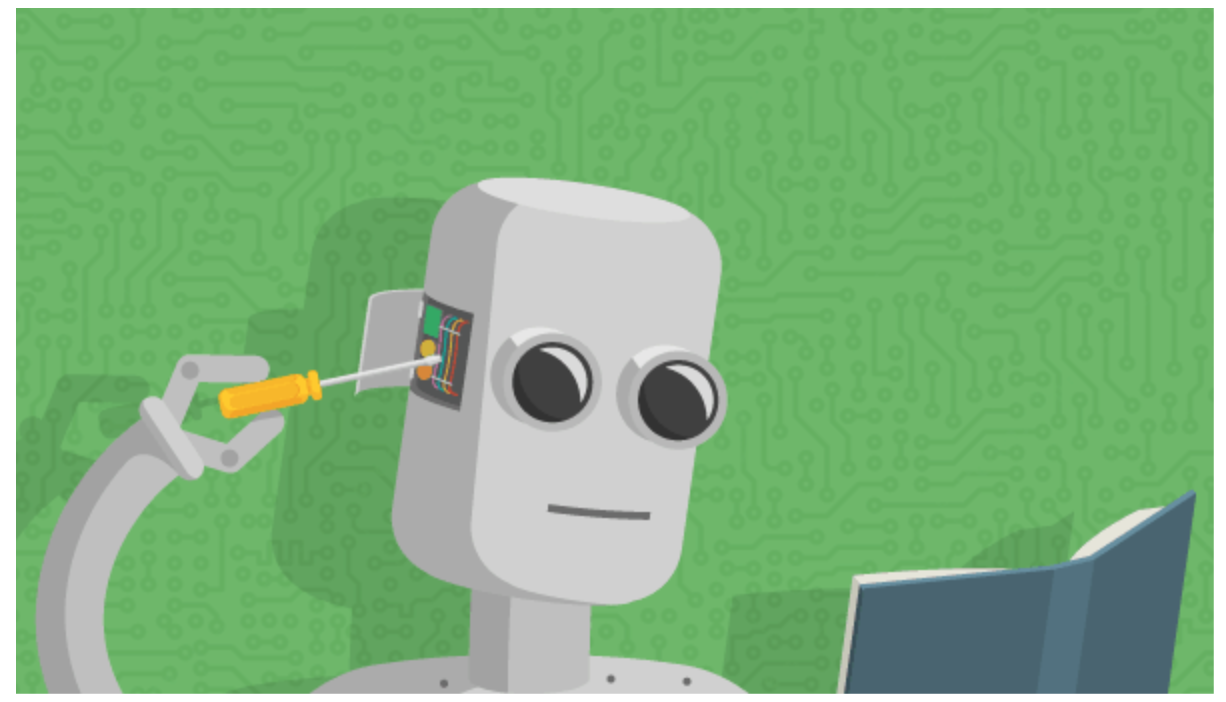
\includegraphics[width=0.5\textwidth]{ml_troll}
	\label{fig:ml_troll}
\end{figure}
Machine Learning is a subfield of Artificial Intelligence that uses statistical techniques to provide computers with the ability to progressively improve performance on different tasks using data, while not being explicitly programmed \cite{wiki:ml}. \\

The application for machine learning are huge and diverse, and range from character recognition to email filtering, with lots of application in computer vision, such as image recognition and classification. \\

Machine learning also focuses on making prediction on data, by utilizing techniques taken from statistics  mathematical optimization. This has many applications, ranging from health care by predicting risk factors for diseases or gaining insights for prevention, to sports or politics where actual results can be predicted.\\

The field of machine learning is subdivided in two broad categories (Fig. \ref{fig:ml_mldiv}), supervised learning (\ref{supervised}) and unsupervised learning (\ref{unsupervised}) (Fig. \ref{unsupervised}) based on whether the data is labeled or not.\\

\begin{figure}[H]
	\centering
	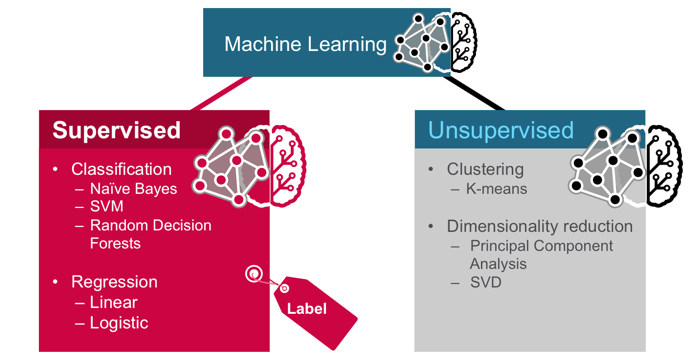
\includegraphics[width=0.75\textwidth]{ml_mldiv}
	\caption{Machine Learning Subfields \cite{ml_mldiv}}
	\label{fig:ml_mldiv}
\end{figure}

Another classification is based on the kind of output that the users wish to obtain, mainly Classification (\ref{classification}), Regression (\ref{regression}) or Clustering.

% TODO: Section or SubSection?
\subsection{Supervised Learning} \label{supervised}
When using supervised learning we want to learn a function that maps an input to an output, based on example input-output pairs \cite{ai_sup}. This means that we need labeled training data, consisting of a vector of input objects and an output value. The objective is to correctly classify the new data based on the previously analyzed training pairs. \\

The general steps to solve a supervised learning problem are (Fig. \ref{fig:sup_wf}):
\begin{enumerate}[noitemsep]
	\item Understand what kind of training example to use.
	\item Gathering a training set.
	\item Model the training set to be fed as input to the algorithm by choosing which features to use and how to represent the data.
	\item Choose what kind of algorithm can best train the model.
	\item Run the algorithm and evaluate the resulting accuracy on the test set 
\end{enumerate}

\begin{figure}[H]
	\centering
	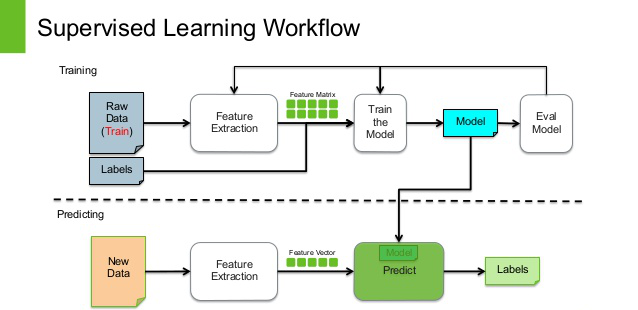
\includegraphics[width=0.5\textwidth]{sup_wf}
	\caption{Supervised Learning Workflow \cite{sup_wf}}
	\label{fig:sup_wf}
\end{figure}

There are important considerations to make when using a supervised learning approach:
\begin{itemize}
	\item \textbf{Dimensionality of Input}: When the input feature vectors are very big there could be problems in learning the function, even if not all features contribute significantly to the function. This happens because the data depends on too many variables and this could cause high variance. \\
	To avoid this, it is important to reduce the number of features through manual removal or using feature selection algorithms. This usually improves the accuracy of the classifier.
	\item \textbf{Overfitting and Underfitting} \cite{overfit}: Overfitting (or overtraining) happens when the algorithm adapts too much on the training data and is no longer able to make accurate predictions on the test data (Fig. \ref{fig:ml_overfit}). This usually happens when there is an excessive number of parameters than can be justified by the data \cite{camb_over}. \\
	Underfitting is the opposite: a model is not able to correctly capture the structure of the data, for example when fitting non linear data with a linear model. \\
	A common way to avoid overfitting is to resample the data using different techniques, commonly k-fold cross validation or leave-one-out. Other methods include feature removal, early stopping, regularization.
	
	\begin{figure}[H]
		\centering
		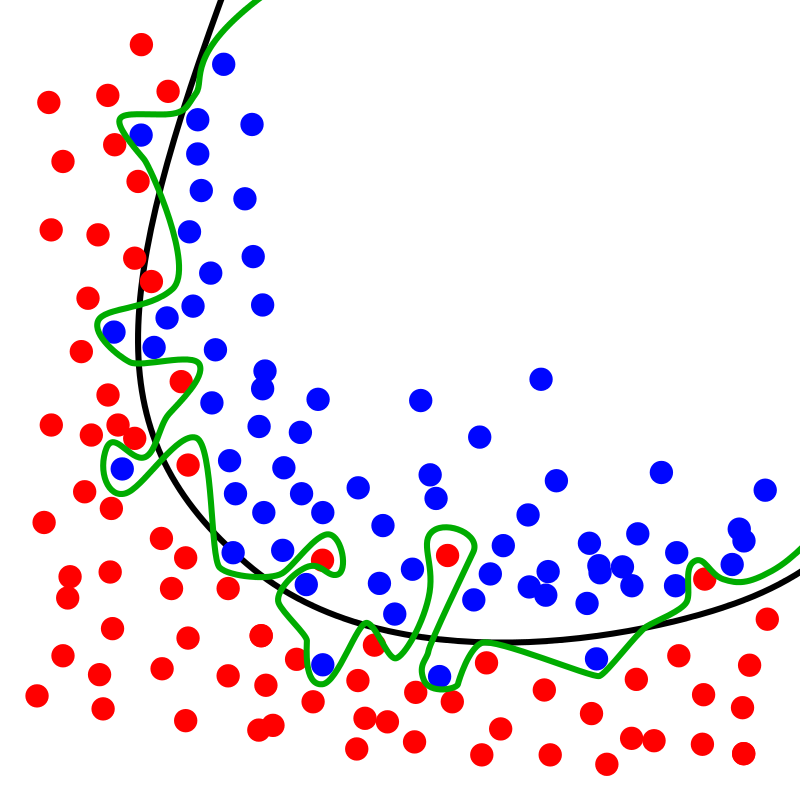
\includegraphics[width=0.5\textwidth]{ml_overfit}
		\caption{Example of Overfitting (green line) \cite{wiki:ml_overfit}}
		\label{fig:ml_overfit}
	\end{figure}	
	
	% TODO: Write this better
	\item \textbf{Bias-Variance Tradeoff} \cite{biasvar}: suppose we have different (but equally good) training set. An algorithm is biased for input $x$ if, when trained on each of these data sets, it is consistently incorrect at predicting the correct output for $x$. \\
	A high bias indicates that the data points tend to be very close to the mean, and to each other.
	A learning algorithm has high variance for a particular input $x$ if it predicts output values that are correct on average but inconsistent when trained on different training sets. \\
	Basically, a high variance indicates that the data points are very spread out from the mean, and from one another.\\
	The prediction error of a classifier is related to the sum of bias and variance, so generally there is a tradeoff between them. Low bias means that it fits the new data well, but if the bias is too low it will fit each training set differently and so result in high variance.\\
	\begin{figure}[H]
		\centering
		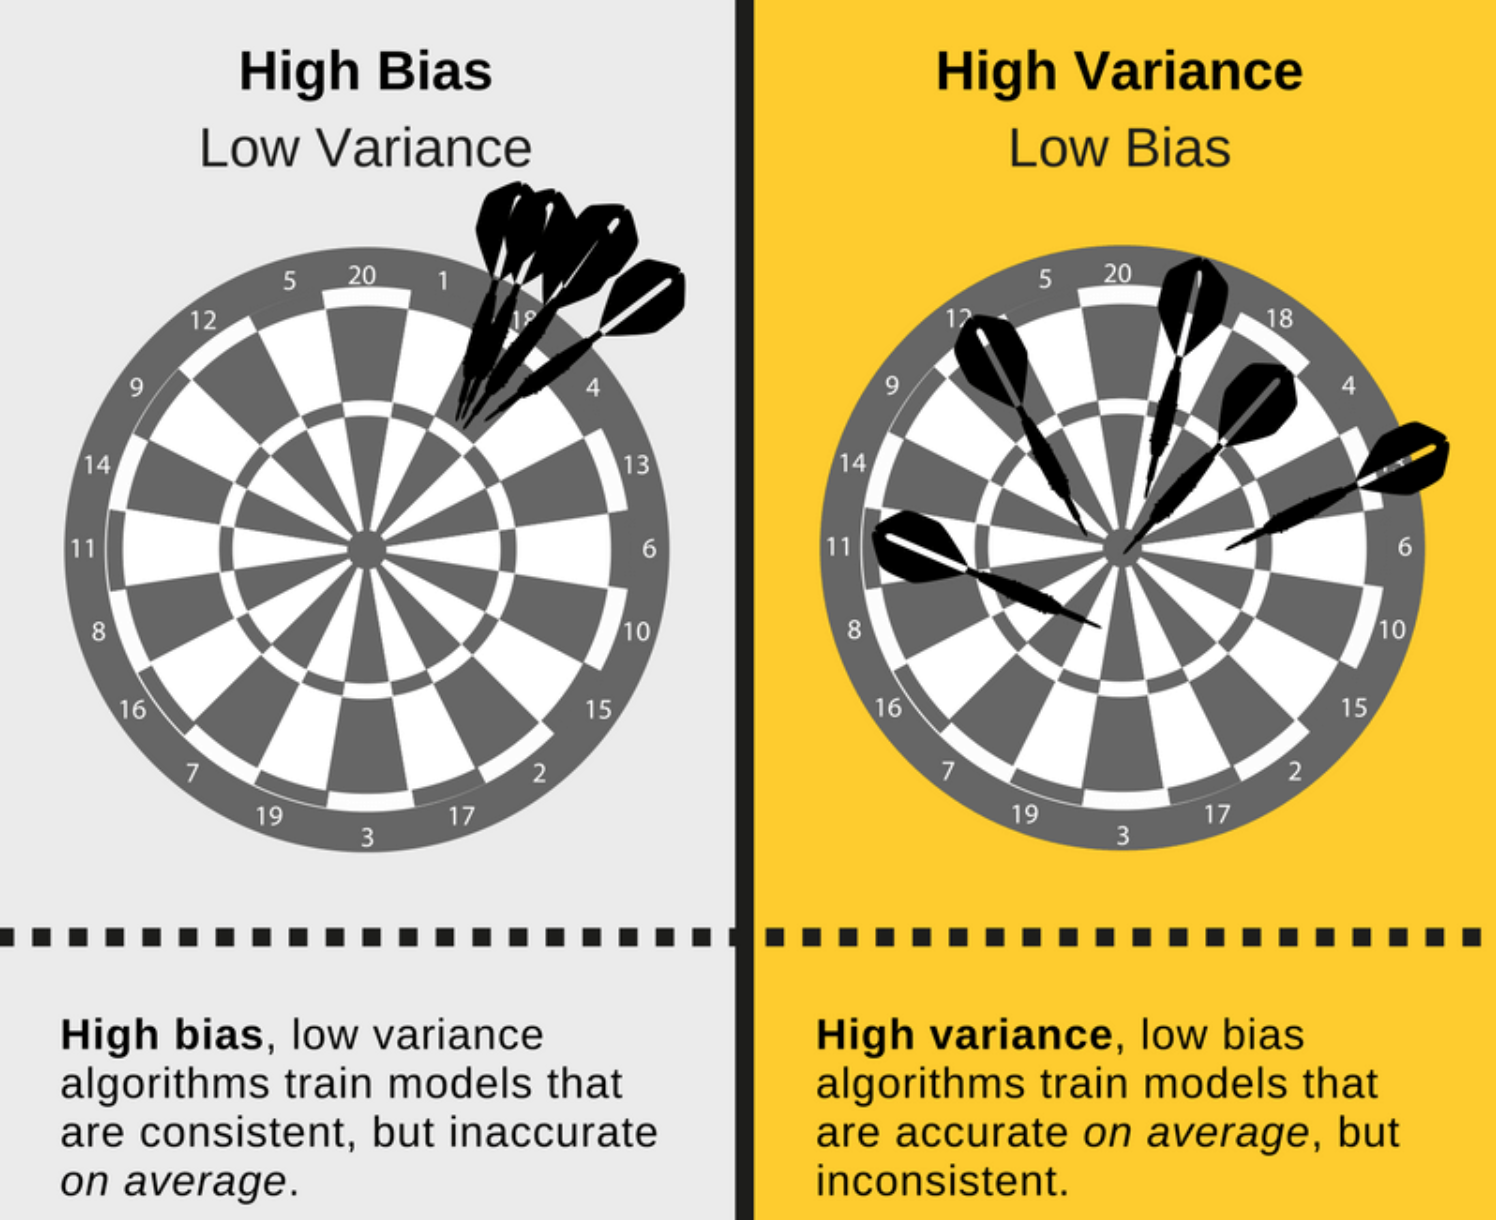
\includegraphics[width=0.5\textwidth]{biasvar}
		\caption{Example of Bias-Variance Tradeoff \cite{biasvarTradeoff}}
		\label{fig:biasvar}
	\end{figure}	
\end{itemize}

There are many algorithms used to perform supervised learning tasks, the most commonly used are: \\
\begin{itemize}[noitemsep, topsep = -5pt]
	\item Linear Regression (\ref{regression})
	\item Logistic Regression
	\item Naive Bayes
	\item Linear Discriminant Analysis
	\item Decision Trees
	\item k-Nearest Neighbor
	\item Neural Networks
	\item Support Vector Machines (\ref{svm})
\end{itemize}

% TODO: Should i write how sup learning works? (from wiki section)

\subsection{Unsupervised Learning} \label{unsupervised}
Unsupervised learning is the subfield of Machine Learning tasked with inferring a function from the analysis of unlabeled data (not classified). Being unclassified there is also a difficulty in to evaluate the accuracy of the model.\\
Usually items are grouped by some measure of similarity, like for example in k-means clustering (Fig. \ref{fig:clustering}).

\begin{figure}[H]
	\centering
	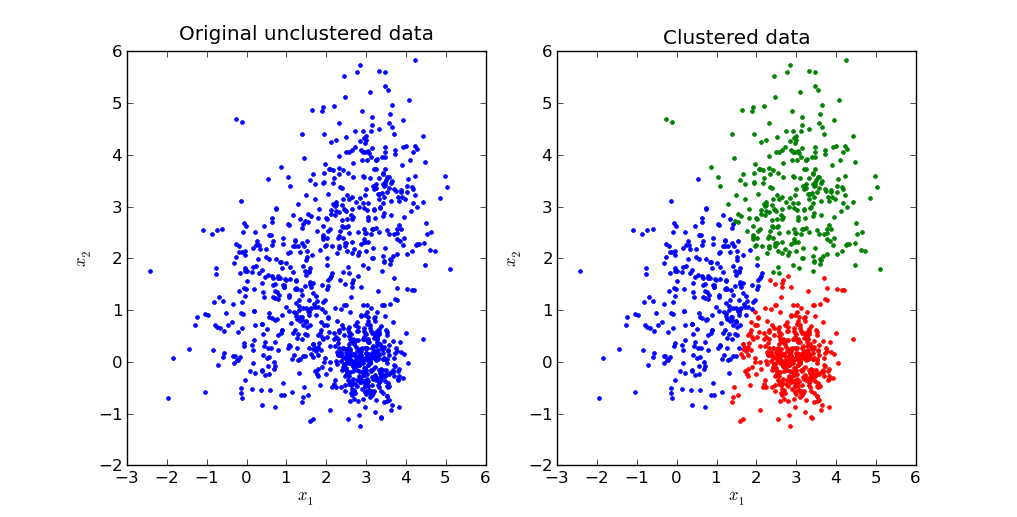
\includegraphics[width=0.5\textwidth]{clustering}
	\caption{Example of Unclustered and Clustered data \cite{kmeans}}
	\label{fig:clustering}
\end{figure}	

These are the most widely used unsupervised learning algorithms:

\begin{itemize}[noitemsep]
	\item Clustering
	\begin{itemize}[noitemsep]
		\item k-means
		\item mixture models
		\item hierarchical clustering
	\end{itemize}
	\item Anomaly detection
	\item Neural Networks
	\begin{itemize}[noitemsep]
		\item Autoencoders
		\item Deep Belief Nets
		\item Hebbian Learning
		\item Generative Adversarial Networks
		\item Self-organizing map
	\end{itemize}
	\item Expectation–maximization algorithm (EM)
	\item Method of moments
	\item Blind signal separation techniques
	\begin{itemize}[noitemsep]
		\item Principal component analysis,
		\item Independent component analysis,
		\item Non-negative matrix factorization
		\item Singular value decomposition.
	\end{itemize}
\end{itemize}

\subsection{Classification} \label{classification}
In machine learning, classification is the problem of identifying in which of a set of categories a new observation belongs, based on a training set of data containing observations whose category is known in advance. A common example is classifying an email as spam or not.\\

Classification is considered an instance of supervised learning, based on instances where a training set is available. As for unsupervised learning, classification would be clustering since it groups data into categories based on similarity, but without knowing the label of the data.\\

The observations, called features or explanatory variables, take different types based on the value. They can be categorical, numerical or ordinal, or be compared by similarity between previous observations using some kind of distance function.\\
The observations representing the categories to be predicted are called explanatory variables (or regressors, or independent variables).\\
The classifier is the algorithm that implements the classification, or a function that maps input data to a category. \\

\begin{figure}[H]
	\centering
	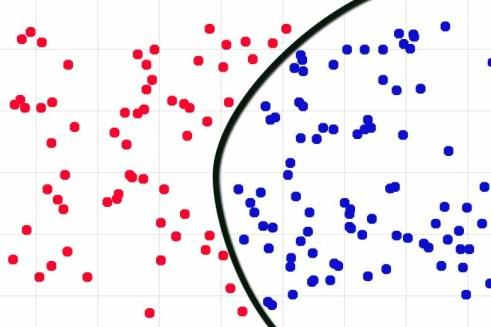
\includegraphics[width=0.5\textwidth]{classification}
	\caption{Example of data division by a Classification algorithm}
	\label{fig:classification}
\end{figure}	

Many classification algorithm, such as SVM (\ref{svm}), logistic regression, LDA (Linear Discriminant Analysis) or perceptron, can be described using a linear function assigning a score to each category c, by doing the dot product of the feature vector of an instance with a vector of weights, thus combining them. The predicted category will be the one with the highest score. This function is called linear predictor function and has this general formula:

\begin{equation}
score(X_i, c) = \beta_c \cdot X_i
\end{equation}

where $X_i$ is the feature vector of instance i and $\beta_c$ is the vector of weights of category c. This kind of algorithms are known as linear classifiers.

\subsection{Regression Analysis} \label{regression}
%TODO: riscrivere e' messo di merda
\begin{figure}[H]
	\centering
	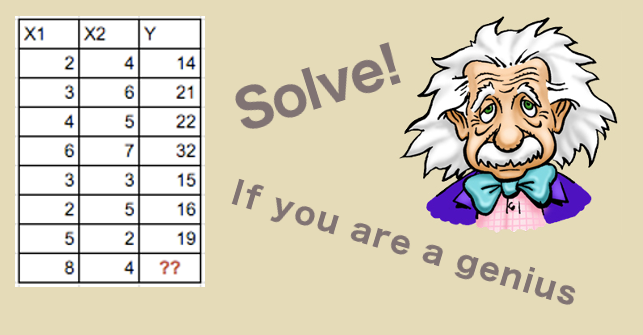
\includegraphics[width=0.5\textwidth]{reg_analysis}
	\caption{Regression Analysis can solve this! \cite{reg_analisys}}
	\label{fig:reg_analysis}
\end{figure}
Regression analysis is used in statistics and machine learning to estimate the relationships between variables. It focus on the relationship between one dependent variable and more independent variables (also called predictors) and it is subsequently used to make predictions on how changing some of the  independent variables will affect the dependent one \cite{wiki:reg_an}. \\

Regression is generally used to estimate the average value of the dependent variable when the independent variables are fixed. In doing that a regression function is calculated. \\
Another use of regression analysis is to understand the relationship among the independent and dependent variables.\\

In regression analysis, it is also of interest to characterize the variation of the dependent variable around the prediction of the regression function using a probability distribution.

\begin{figure}[H]
	\centering
	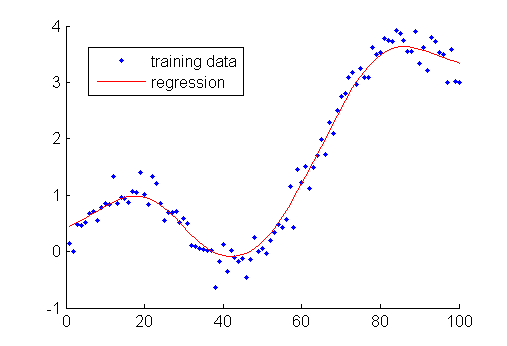
\includegraphics[width=0.5\textwidth]{reg_plot}
	\caption{Example of Regression Analysis}
	\label{fig:reg_plot}
\end{figure}	

\subsubsection*{Regression Model} 
A general regression model uses the following variables and parameters:
The unknown parameters, $\beta$, that represents either a scalar or a vector.\\
The independent variables, $X$. \\
The dependent variable, $Y$.\\

A regression model relates $Y$ to a function of $X$ and $\beta$.
\begin{equation}
	Y \approx f(X,\beta)
\end{equation}

This is usually formalized as
\begin{equation}
	E(Y|X) = f(X,\beta)
\end{equation}

%TODO: riguardare anche questo, troppo wiki
If $\beta$ is of length $k$ and the number of observed data points is enough ($N > k$), then it's possible to estimate a unique value for $\beta$ that best fits the data. \\

If this is the case, regression analysis provides the means to find a solution for unknown parameters of $\beta$ to, for example, apply the method of least squares.

To apply regression the data must abide by some assumption, generally:
\begin{itemize}[noitemsep, topsep = -5pt]
	\item The sample is representative of the population for the inference prediction.
	\item The error is a random variable with a mean of zero.
	\item The independent variables are measured with no error.
	\item The independent variables (predictors) are linearly independent.
	\item The errors are uncorrelated.
	\item The variance of the error is constant across observations.
\end{itemize}

%TODO: section or sub?
\subsection{Linear Regression} \label{lin_reg}
Linear regression is the most basic case of Regression Analysis, and it is a useful tool for predicting a quantitative response. Also, most of the newer approaches to regression are often a generalization or extension of linear regression. \\

Linear regression is a linear approach to modeling the relationship between a dependent variable and one or more independent variables. The simplest case of linear regression (LR) is when there is only one independent variable, and is called simple linear regression \cite{wiki:lin_reg} and has this form:
\begin{equation}
	y_i \approx \beta_0 + \beta_1x_i + \varepsilon_i
\end{equation}
where $\epsilon_i$ is the error for the i-th observation. The error is a catch-all for what we miss with this simple model, since it's very probable that the true relationship is not linear, and that there may be other variables that influence $y$. \\

The point of LR is to estimate the $\beta$ coefficients to make predictions. To do so, we utilize of the training dataset to produce estimates $\widehat{\beta_0}$ and $\widehat{\beta_1}$ for the model coefficients. We can then make predictions by computing:
\begin{equation}
\widehat{y_i} \approx \widehat{\beta_0} + \widehat{\beta_1x_i}
\end{equation}

$e_i = y_i - \widehat{y_i}$ is the difference between the true value and the prediction for an observation, and it is called residual (Fig. \ref{fig:reg_error}). \\

\begin{figure}[H]
	\centering
	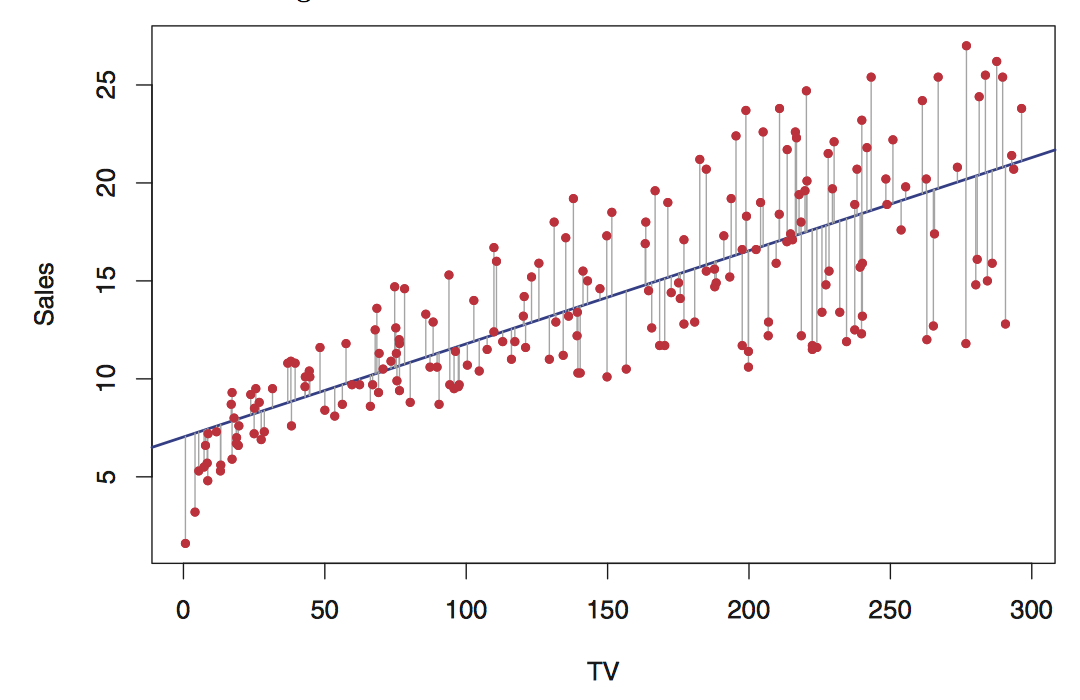
\includegraphics[width=0.5\textwidth]{reg_error}
	\caption{The fit is found by minimizing the sum of squared errors. Each gray line segment represents an error, and the prediction makes a compromise by averaging their square \cite{ISLR}}
	\label{fig:reg_error}
\end{figure}

The most common method for estimation is called least squares. This method obtains parameter estimates that minimize the sum of squared residuals (SSR):
\begin{equation}
	SSR=\sum _{i=1}^{n}e_{i}^{2}
\end{equation}

The minimizers are
\begin{equation}
	 \widehat{\beta_{1}} = \frac{\sum(x_i - \bar{x})(y_i - \bar{y})}{\sum(x_i - \bar{x})^2}
\end{equation}
\begin{equation}
	\widehat{\beta_{0}} = \bar{y} - \widehat{\beta_{1}} \bar {x}
\end{equation}

where $\bar{x}$ and $\bar{y}$ are the mean of $x$ and $y$.\\

If we assume that the error term has constant variance, the estimate of the variance of the error is given by:

\begin{equation}
	\widehat{\sigma}_{\varepsilon }^{2} = \frac{SSR}{n-2}
\end{equation}

And is called mean square error (MSE) of the regression. The denominator is the sample size reduced by the number of model parameters estimated from the same data, $(n-p)$ for $p$ regressors or  $(n-p-1)$ if an intercept is used \cite{MSE}. In the case of simple linear regression $p=1$, so the denominator is $n-2$.

We can then estimate the standard errors for the parameters, that tell us the average amount that the estimate differs from the actual value.
\begin{equation}
	{\widehat{\sigma}_{\beta _{1}} = {\widehat{\sigma}_{\varepsilon}{\sqrt{\frac{1}{\sum(x_{i} - {\bar {x}})^{2}}}}}}
\end{equation}
\begin{equation}
	{\widehat{\sigma}_{\beta _{0}} = {\widehat{\sigma}_{\varepsilon}{\sqrt{\frac{1}{n} + \frac{\bar{x}^2}{\sum(x_{i} - {\bar {x}})^{2}}}}}}
\end{equation}

Standard errors can be used to compute confidence intervals. A 95\% confidence interval is defined as a range of values such that with 95\% probability, the range will contain the true unknown value of the parameter.

The general multiple regression model, where there are $p$ independent variables, follows this formula:
\begin{equation}
	y_{i}=\beta_{1}x_{i1} + \beta_{2}x_{i2} + \cdots + \beta_{p}x_{ip} + \varepsilon_{i}
\end{equation}
where $x_{ij}$ is the i-th observation on the j-th independent variable.



\pagebreak

\section{Logistic Regression}
In regression analysis, logistic regression is a method for estimating the parameters of a logistic model. A logistic model is one where the log-odds of the probability of an event is a linear combination of independent or predictor variables. \\
The two possible dependent variable values are often labeled as "0" and "1", "true" or "false", "pass" or "fail" etc, and they represent binary outcomes (Fig. \ref{fig:logistic_exam}). \\
It's possible to generalize the binary logistic regression model to more than two levels (outcomes) of the dependent variable \cite{wiki:logisticreg}.

The binary logistic model works by estimating the probability of a binary response based on one or more predictor variables.\\
With logistic regression is possible to say how much that the presence of a risk factor increases the odds of a given outcome. \\
The model itself simply calculates the probability of output in terms of input, and it is not specifically a classifier, but it can be used to classify data by choosing a threshold value, for example if the probability is $\ge 50\%$ the class is "1" otherwise is "0".

\begin{figure}[H]
	\centering
	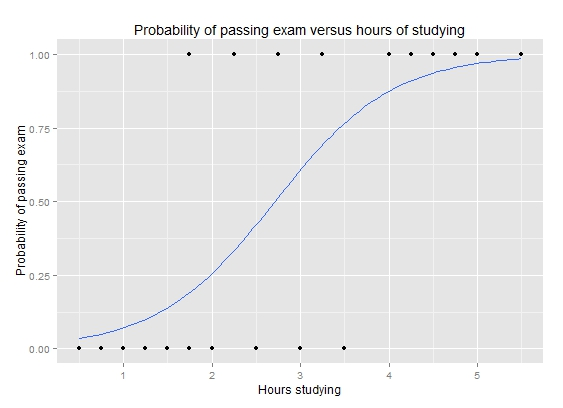
\includegraphics[width=0.5\textwidth]{exam_pass_logistic_curve}
	\caption{Graph of a logistic regression curve showing probability of passing an exam versus hours studying \cite{wiki:logisticreg}}
	\label{fig:logistic_exam}
\end{figure}

\subsubsection{Logistic Function}
The logistic function to estimate the probabilities is a sigmoid function (exemplified in fig. \ref{fig:sigmoid}). \\
A sigmoid function takes an input from the real numbers and outputs a value between $0$ and $1$.

\begin{figure}[H]
	\centering
	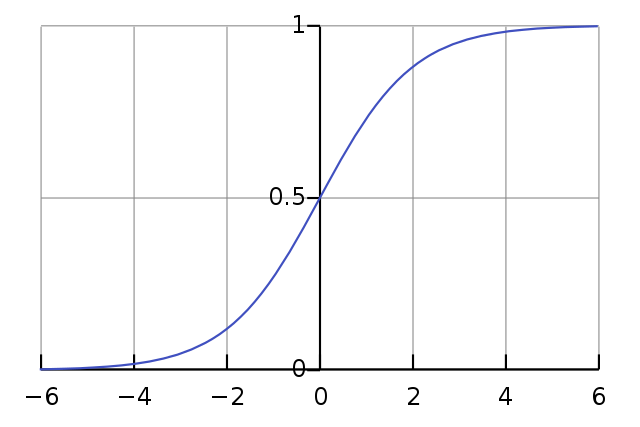
\includegraphics[width=0.5\textwidth]{sigmoid}
	\caption{Example of a Sigmoid shaped function}
	\label{fig:sigmoid}
\end{figure}

We want to model the relationship between $p(X) = Pr(Y = 1|X)$ and $X$. To model this relationship we use the a logistic function:

\begin{equation} \label{eq:logr1}
		p(X) = \frac{e^{\beta_{0}} + e^{\beta_{1}X}}{1+ e^{\beta_{0}} + e^{\beta_{1}X}} = \frac{1}{1 + e^{-({\beta_{0} + \beta_{1}X})}}
\end{equation} 

Equation \ref{eq:logr1} can be manipulated into: 

\begin{equation} \label{eq:logr2}
	\frac{p(X)}{1 - p(X)} = e^{\beta_{0}} + e^{\beta_{1}X}
\end{equation} 

$\frac{p(X)}{1 - p(X)}$ is called odds, and can take any value between $0$ and $\infty$.

By doing the logarithm of \ref{eq:logr2} we get:

\begin{equation} \label{eq:logr3}
	\log{\frac{p(X)}{1 - p(X)}} = \beta_{0} + \beta_{1}X
\end{equation} 

The coefficients $\beta_{0}$ and $\beta_{1}$ in equation \ref{eq:logr1} are unknown, and must be estimated based on the available training data. \\
To fit the model of equation \ref{eq:logr3}, the maximum likelihood method is commonly used. \\
Intuitively we want to estimates $\beta_{0}$ and $\beta_{1}$ such that the predicted probability ${\hat{p}}(x_i)$ for a specific case corresponds as closely as possible to the observed class for that case.\\
This can be achieved by using the likelihood function:

\begin{equation} \label{eq:logr4}
	\ell(\beta_{0}, \beta_{1}) = \prod_{i:y_i = 1}p(x_i) \prod_{i':{y_{i'}} = 0} (1- p(x_{i'}))
\end{equation} 

The estimates $\hat{\beta_{0}}$ and $\hat{\beta_{1}}$ are chosen to maximize this likelihood function.\\
Maximum likelihood is a very general approach that is used to fit many of the non-linear models. For example in linear regression (Ch. \ref{lin_reg}), the least squares approach is a special case of maximum likelihood.

Once the coefficient have been estimated is pretty simple to compute the probability:
\begin{equation}
	\hat{p}(X) = \frac{e^{\hat{\beta_{0}}} + e^{\hat{\beta_{1}}X}}{1+ e^{\hat{\beta_{0}}} + e^{\hat{\beta_{1}}X}}
\end{equation}

\pagebreak

\section{Random Forest}
%TODO: review from wiki

\begin{figure}[H]
	\centering
	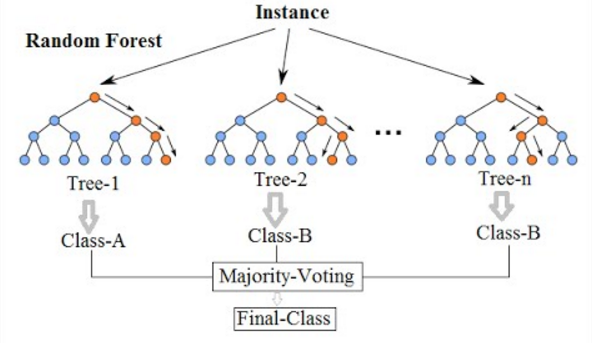
\includegraphics[width=0.7\textwidth]{RFClass}
	\caption{Example of Random Forest Classification \cite{medium:RF}}
	\label{fig:RFClass}
\end{figure}

Random forests are an ensemble learning method used mainly for classification and regression. They work by building a lot of decision trees while training, and outputting the class that is the mode of the classes for classification, or the mean prediction of the individual trees for regression \cite{wiki:randomforest}. \\

Random Forest (RF) is preferred to decision trees because decision trees suffer from high variance. By using tree bagging, which is a commonly used technique to reduce variance, we can correct decision trees' habit of overfitting to their training set \cite{ESL}.

\subsubsection{Decision Trees}

\begin{figure}[H]
	\centering
	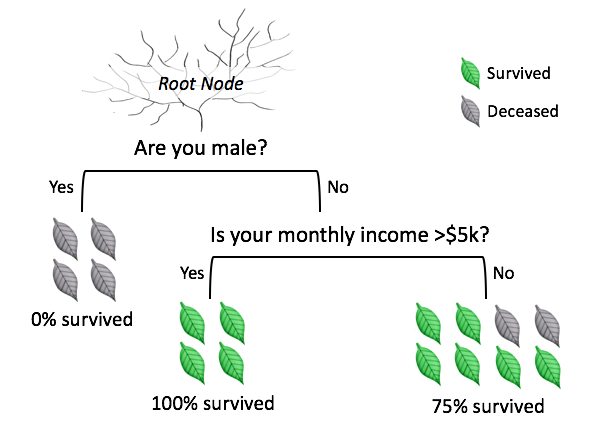
\includegraphics[width=0.7\textwidth]{decTree}
	\caption{Example of a Decision Tree \cite{KDNrf}}
	\label{fig:decTree}
\end{figure}

Decision trees are a popular method for various machine learning tasks and can be used for either classification or regression. However, they are often inaccurate. Specifically, by growing trees very deep, they tend to learn highly irregular patterns by overfitting to the training set (i.e. have low bias, but very high variance). \\
Random forests are a way of averaging multiple deep decision trees, trained on different parts of the same training set, with the goal of reducing the variance. \\
This comes at the expense of a small increase in the bias and some loss of interpretability, but generally greatly boosts the performance in the final model \cite{ESL}. 

\subsubsection{Tree Bagging}
Given a set of $n$ independent observations $X_1, \dots, X_n$, each with variance $\sigma^2$, the variance of the mean $\overline{X}$ of the observations is given by $\sigma^2/n$. \\
This means that averaging a set of observations reduces the variance. So to reduce the variance we can take many training sets from the population, build a prediction model using each training set, and average the resulting predictions. \\
Basically we could calculate $\hat{f}^1(x), \hat{f}^2(x), \dots, \hat{f}^B(x)$ using B separate training sets, and average them in order to obtain a single model with low-variance \cite{ISLR}. \\

This solution is not practical since we normally lack more than one training set. \\
Instead we utilize bagging: we can take repeated samples from the training set in order to generate B different bootstrapped training sets. We then train our method on the $b_{th}$ bootstrapped training set, and then average the resulting predictions. \\

To apply bagging to regression trees specifically, we simply construct B regression trees using B bootstrapped training sets, and average the resulting predictions. These trees are grown deep, and are not pruned. Hence each individual tree has high variance, but low bias. Averaging these B trees reduces the variance \cite{ISLR}. \\

If we are using RF for classification (like in this thesis), the simplest approach is the following: \\
Given test observation, we record the class predicted by each of the $B$ trees, and take a majority vote: the final prediction is the most frequent class among the $B$ predictions. \\

More formally, given a training set $X = x_1, \dots, x_n$ with responses $Y = y_1, \dots, y_n$, bagging $B$ times selects a random sample with replacement of the training set and fits trees to these samples \cite{wiki:randomforest}: \\

For $b = 1, \dots, B$:
\begin{enumerate}[noitemsep]
	\item Sample, with replacement, $n$ training examples from $X, Y$; call these $X_b, Y_b$.
	\item Train a classification or regression tree $f_b$ on $X_b, Y_b$.
\end{enumerate}

After training, predictions for unseen samples $x'$ can be made by averaging the predictions from all the individual regression trees on $x'$:

\begin{equation}
	{{\hat {f}}={\frac {1}{B}}\sum _{b=1}^{B}f_{b}(x')}
\end{equation}

or by using the majority vote in case of classification.\\
%TODO: from here
%todo : maybe remove the rest
Additionally, an estimate of the uncertainty of the prediction can be made as the standard deviation of the predictions from all the individual regression trees on $x'$:

\begin{equation}
	{\sigma ={\sqrt {\frac {\sum_{b=1}^{B}(f_{b}(x')-{\hat {f}})^{2}}{B-1}}}}
\end{equation}

The number of samples/trees, B, is a free parameter. Typically, a few hundred to several thousand trees are used, depending on the size and nature of the training set. \\
An optimal number of trees B can be found using cross-validation, or by observing the out-of-bag error: the mean prediction error on each training sample $x_i$, using only the trees that did not have $x_i$ in their bootstrap sample. \\
The training and test error tend to level off after some number of trees have been fit \cite{ISLR}.

\subsubsection{From Bagging to Random Forests}

%todo: change caption
\begin{figure}[H]
	\centering
	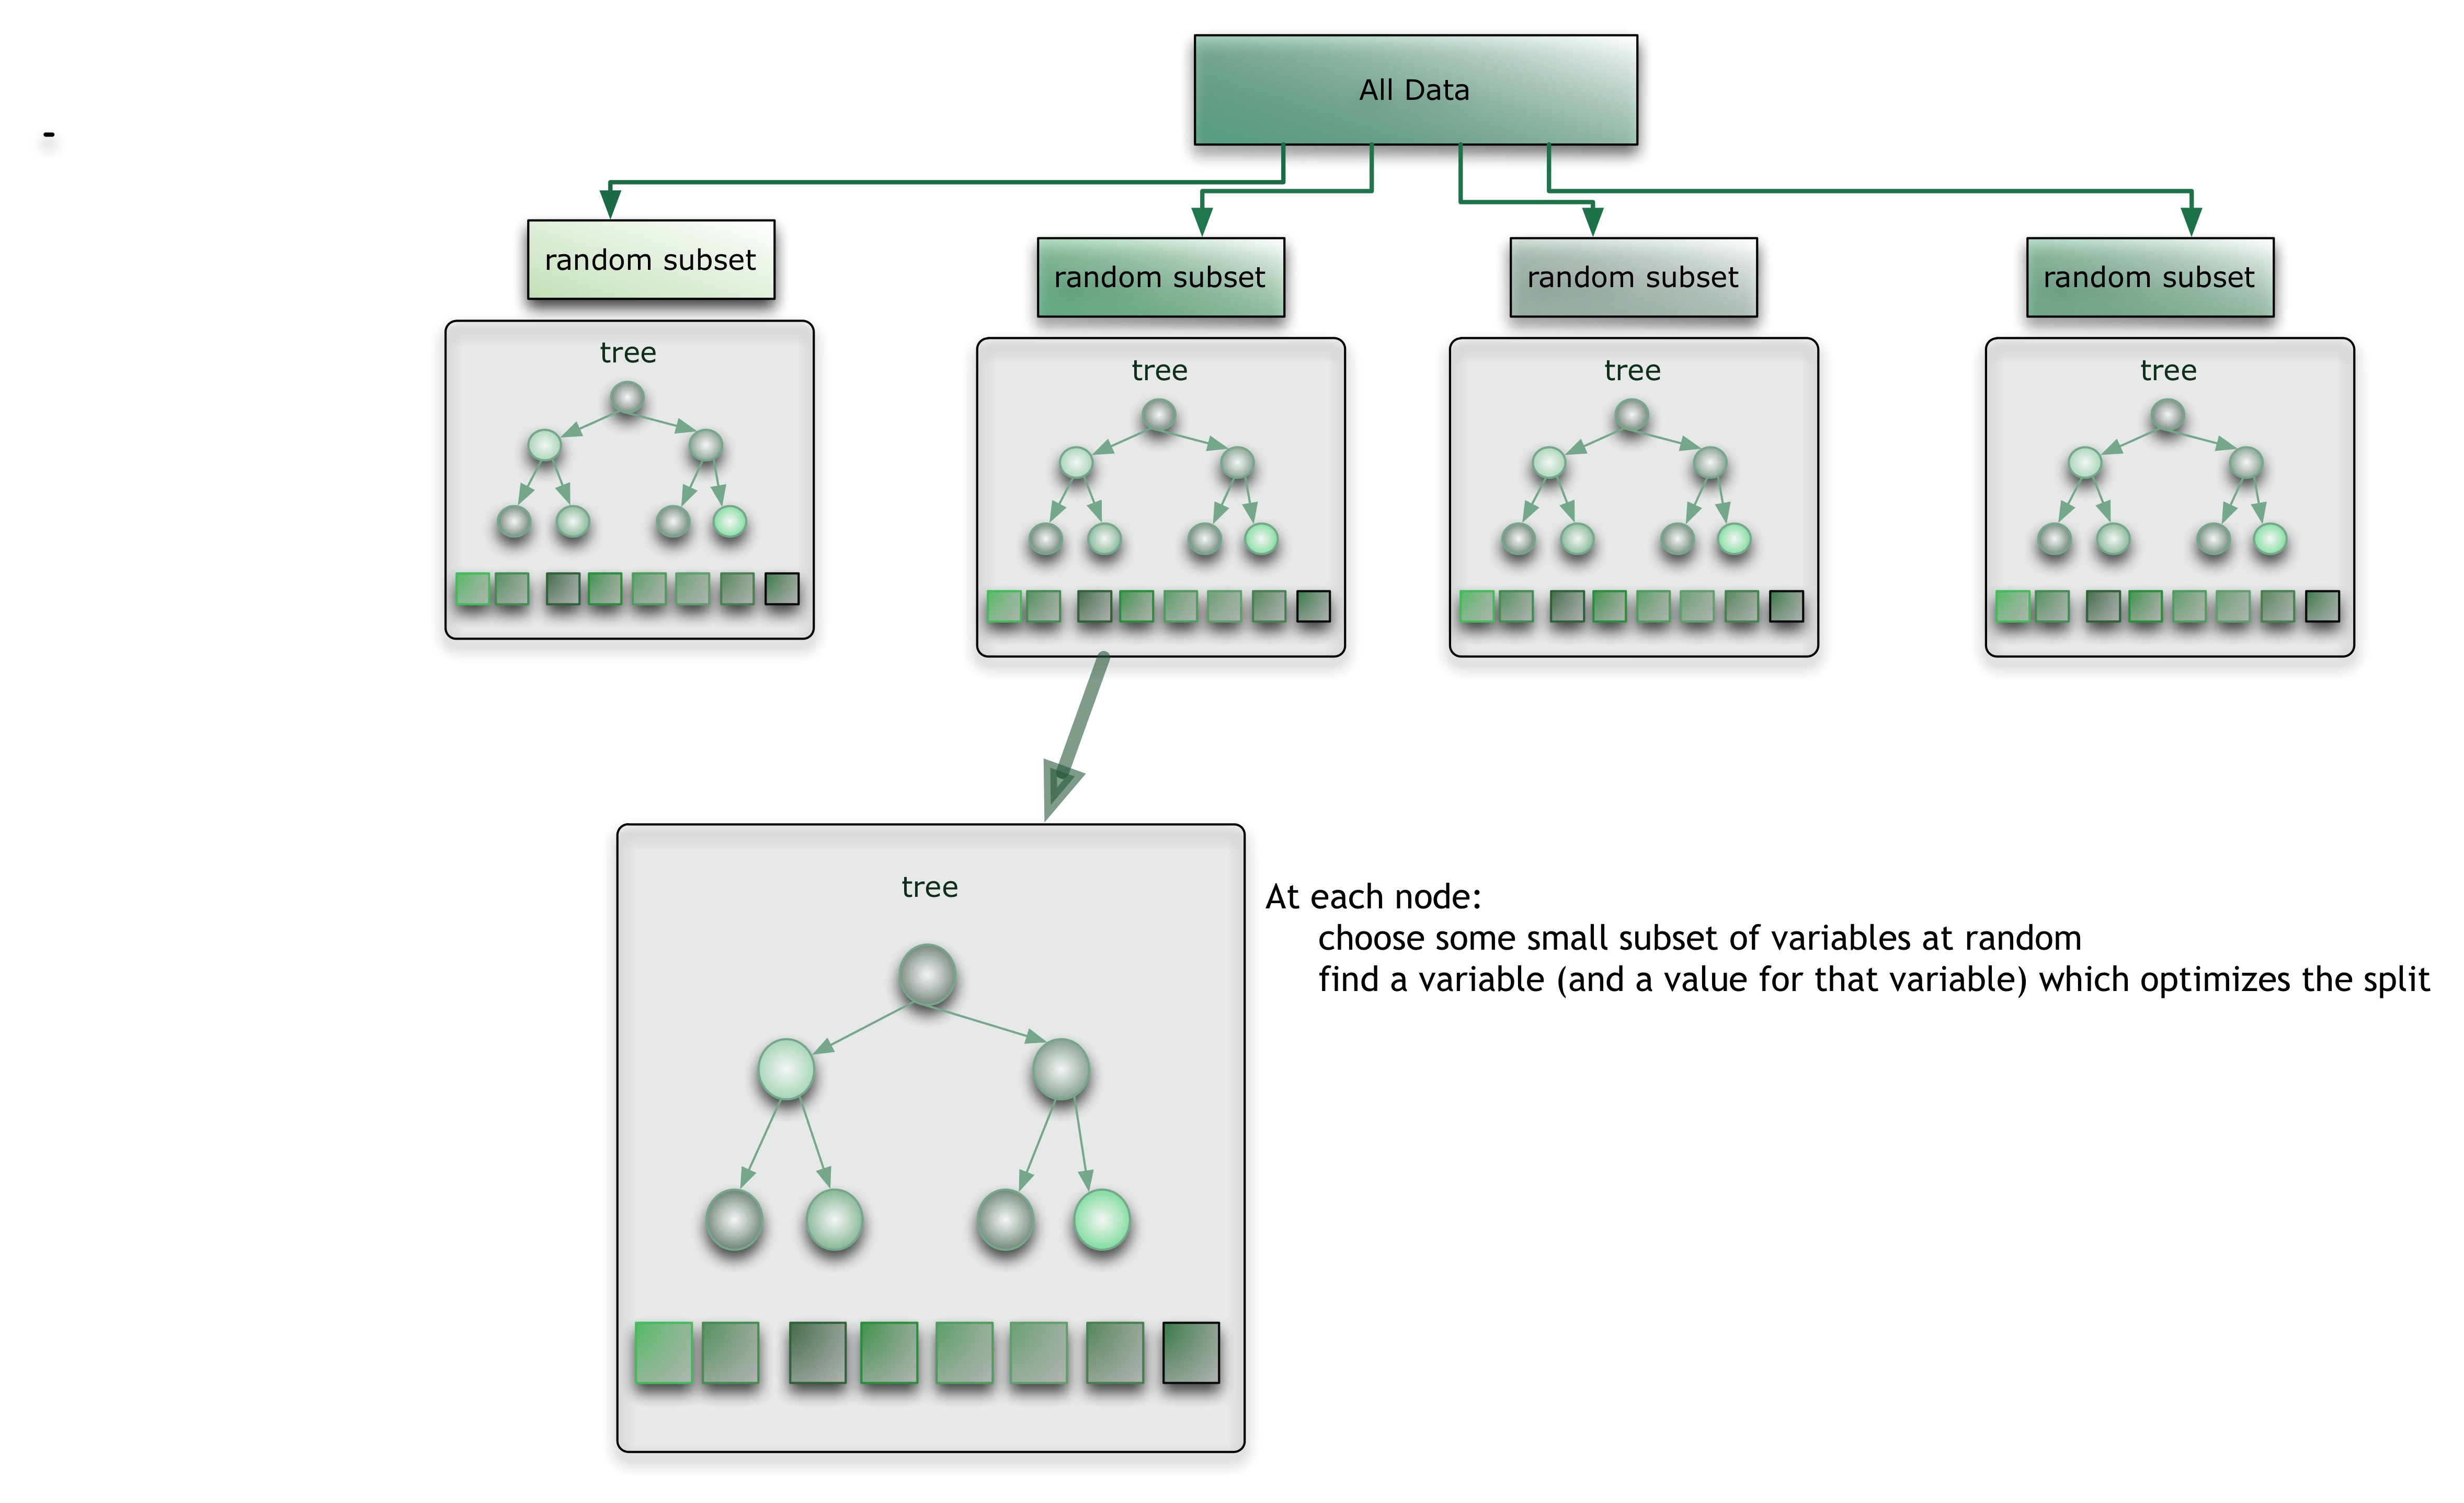
\includegraphics[width=0.7\textwidth]{RF}
	\caption{Random Forest overview}
	\label{fig:RF}
\end{figure}

Random Forests provide an improvement over bagged decision trees by decorrelating the trees. As in bagging, the decision trees are built on a bootstrapped training set. The difference is that every time a split is considered, a random sample of $m$ predictors is chosen as split candidates from the total $p$ predictors. The split can only use one of those $m$ predictors. $\sqrt{m}$ predictors are taken each split, typically with $m \equiv \sqrt{p}$ \cite{ISLR}.\\

Practically, at each split in the tree, the algorithm can only consider a subset of the predictors. This works because if there is a very strong predictor, that predictor would be used in the majority of the trees, and then all the bagged trees would look alike and highly correlated, thus leading to a small reduction in variance.\\

By forcing each split to consider only $m$ predictors, on average $(p - m)/p$ of splits will not take into account a strong predictor. This, in turn, will decorrelate the trees.\\

\pagebreak

\section{SVM} \label{svm}
Support Vector Machines (SVM) are a supervised machine learning algorithm used for both classification and regression. \\

The main idea is to find the optimal hyperplane for linearly separable data, and then extend this idea to data that are not linearly separable, by mapping this data in a new space using a kernel function.\\

The definition of an hyperplane for p-dimensions is:
\begin{equation}
\beta_0 + \beta_1 X_1 + \beta_2 X_2 + \dots + \beta_p X_p = 0
\end{equation}

Support vectors are the data points that lie closest to the hyperplane (Fig. \ref{fig:suppvec}), they also are the data points most difficult to classify and have direct bearing on the optimum location of the hyperplane.\\
\begin{figure}[h]
	\centering
	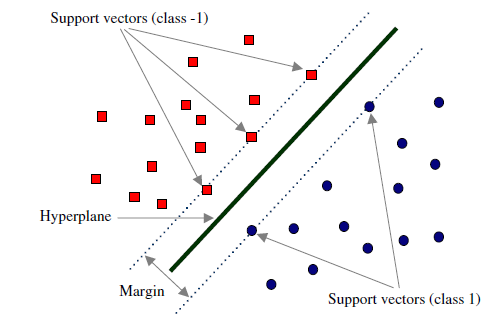
\includegraphics[width=0.5\textwidth]{svm_support_vectors}
	\caption{Example of Support Vectors}
	\label{fig:suppvec}
\end{figure}

The distance between the hyperplane and the nearest data point from either set is known as the margin. The best hyperplane is the one that maximizes the margins for the data we are classifying.\\
\begin{figure}[H]
	\centering
	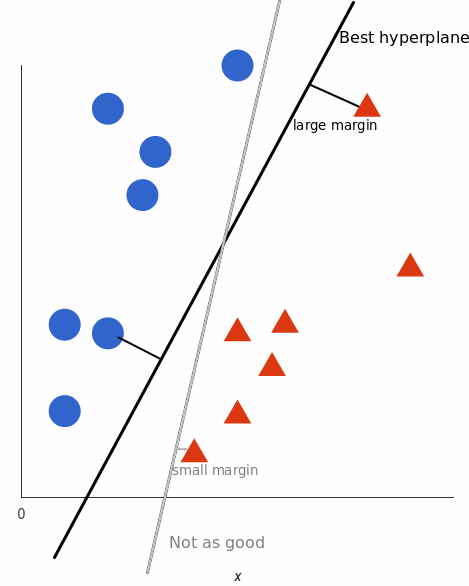
\includegraphics[width=0.5\textwidth]{hyperplane_margin}
	\caption{Different hyperplanes with different margins \cite{svm_monkeylearn}}
\end{figure}

So the objective is to choose a hyperplane with the largest possible margin between it and the support vectors, since the larger is the margin, the lower the generalization error of the classifier.\\

In essence, support vectors are the elements of the training set that would change the position of the dividing hyperplane if removed. This makes the support vectors the critical elements of the training set.\\

Finding the maximal margin hyperplane based on a set of training observations $x_1, \dots x_n \in R^p$ and with class lables $y_1 \dots y_n$, translates to an optimization problem:\\

Maximize M
\begin{equation} \label{eq:svm1}
\beta_0, \beta_1, \beta_2, \dots, \beta_p, M
\end{equation}

subject to
\begin{equation} \label{eq:svm2}
\sum_{j=1}^{p}\beta^2_j = 1
\end{equation}

\begin{equation} \label{eq:svm3}
y_i(\beta_0 + \beta_1 X_i1 + \beta_2 X_i2 + \dots + \beta_p X_ip) \ge M \quad \forall i = 1, \dots, n
\end{equation}

\ref{eq:svm2} and \ref{eq:svm3} ensure that each observation is on the correct side of the hyperplane and at least a distance M from the hyperplane. Hence, M represents the margin of our hyperplane, and the optimization problem chooses $\beta_0, \beta_1, \beta_2, \dots, \beta_p$ to maximize M. \\

Unfortunately this hyperplane does not necessarily exists, but we can extend this concept to find a hyperplane that almost separates the classes using a soft margin. This is what an really SVM does.

It is very probable that the data is not linearly separable, as we can see in figure \ref{fig:svmnotsep}:
\begin{figure}[H]
	\centering
	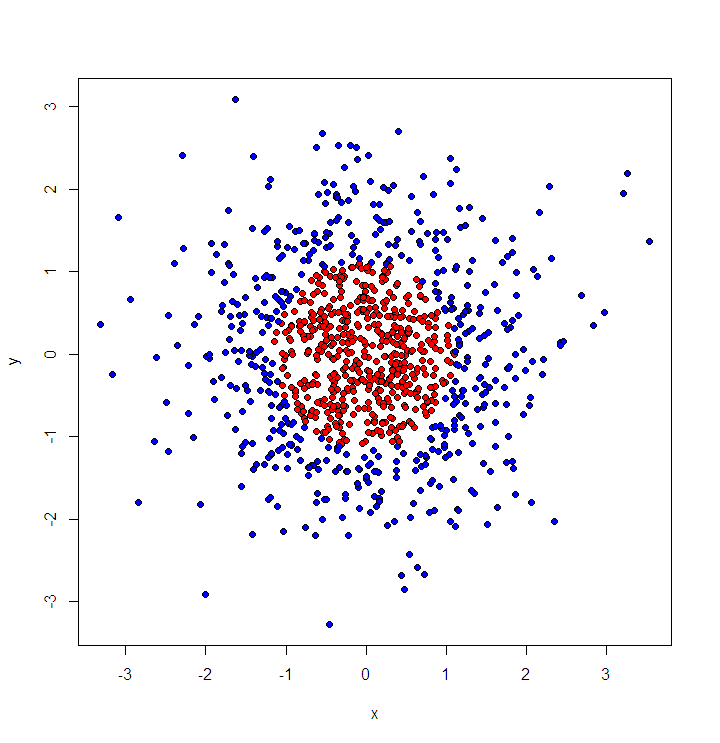
\includegraphics[width=0.5\textwidth]{svm_not_separable}
	\caption{Linearly not separable data \cite{svm_monkeylearn}}
	\label{fig:svmnotsep}
\end{figure}

In this case, for example, we can add a new dimension and separate the data. 
\begin{figure}[H]
	\centering
	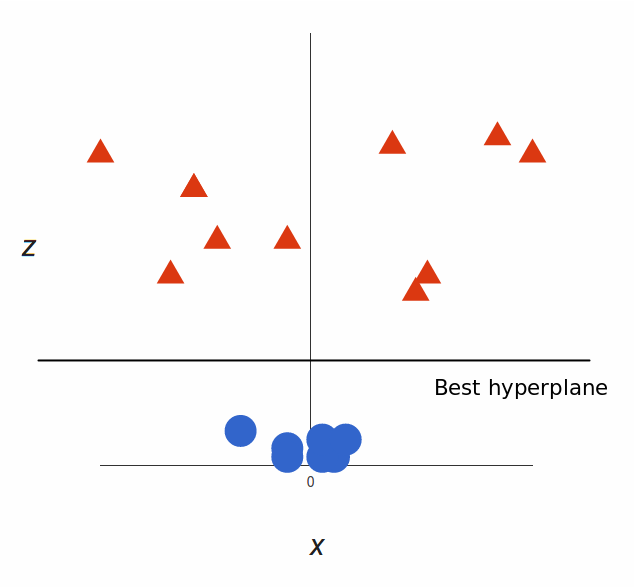
\includegraphics[width=0.5\textwidth]{svm_three_dim}
	\caption{Three dimensional separable space \cite{svm_monkeylearn}}
\end{figure} 

And then map back to two dimensions.
\begin{figure}[H]
	\centering
	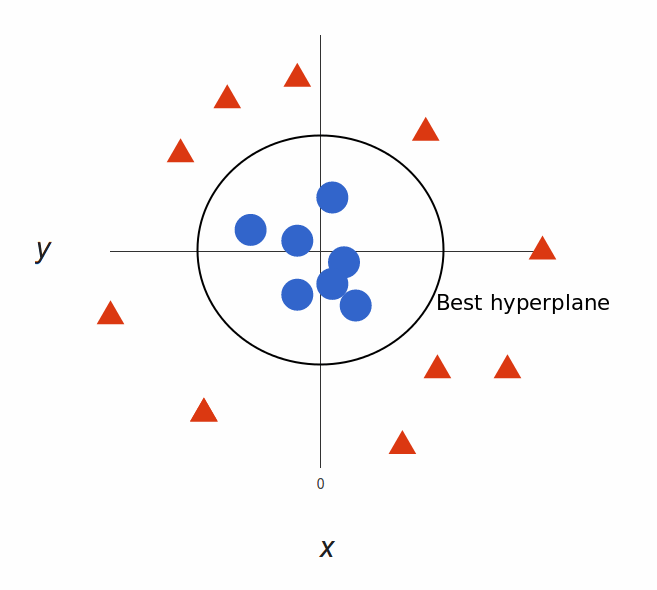
\includegraphics[width=0.5\textwidth]{svm_separated}
	\caption{Separated data \cite{svm_monkeylearn}}
\end{figure}

Calculating the transformation can be very computationally intensive, but SVM just needs the dot product between the vectors. This is called the kernel function. Kernels can be of different types, like linear or 
